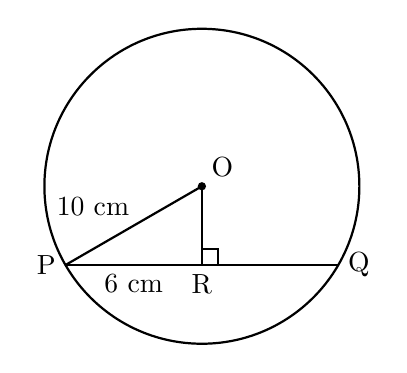
\begin{tikzpicture}[scale=1]

  % Define the center of the circle
  \coordinate (O) at (0,0);

  % Define the radius of the circle
  \def\R{2}

  % Draw the circle
  \draw[thick] (O) circle (\R);

  % Add a dot at the center
  \fill (O) circle (1.5pt);

  % Add the label 'O' near the center
  \node[above right] at (O) {O};

  % Define coordinates for points P, R, and Q
  % They lie on a horizontal chord below the center
  % Let the y-coordinate be around -1
  % Then x^2 + (-1)^2 = 2^2 => x^2 = 3 => x = sqrt(3) ~= 1.732
  \coordinate (P) at (-1.732, -1);
  \coordinate (Q) at (1.732, -1);
  \coordinate (R) at (0, -1);

  % Draw the line segment PQ (chord)
  \draw[thick] (P) -- (Q);

  % Draw the line segment OP (radius)
  \draw[thick] (O) -- (P);

  % Draw the line segment OR (perpendicular from center to chord)
  \draw[thick] (O) -- (R);

  % Add labels for the points P, R, and Q
  \node[left] at (P) {P};
  \node[below] at (R) {R};
  \node[right] at (Q) {Q};

  % Add the right-angle symbol at R
  \draw[thick] (0, -0.8) -- (0.2, -0.8) -- (0.2, -1);

  % Add measurement labels
  \node[above left] at (-0.8, -0.5) {10 cm};
  \node[below] at (-0.866, -1) {6 cm};

\end{tikzpicture}